\begin{figure}[h]
    \begin{center}
    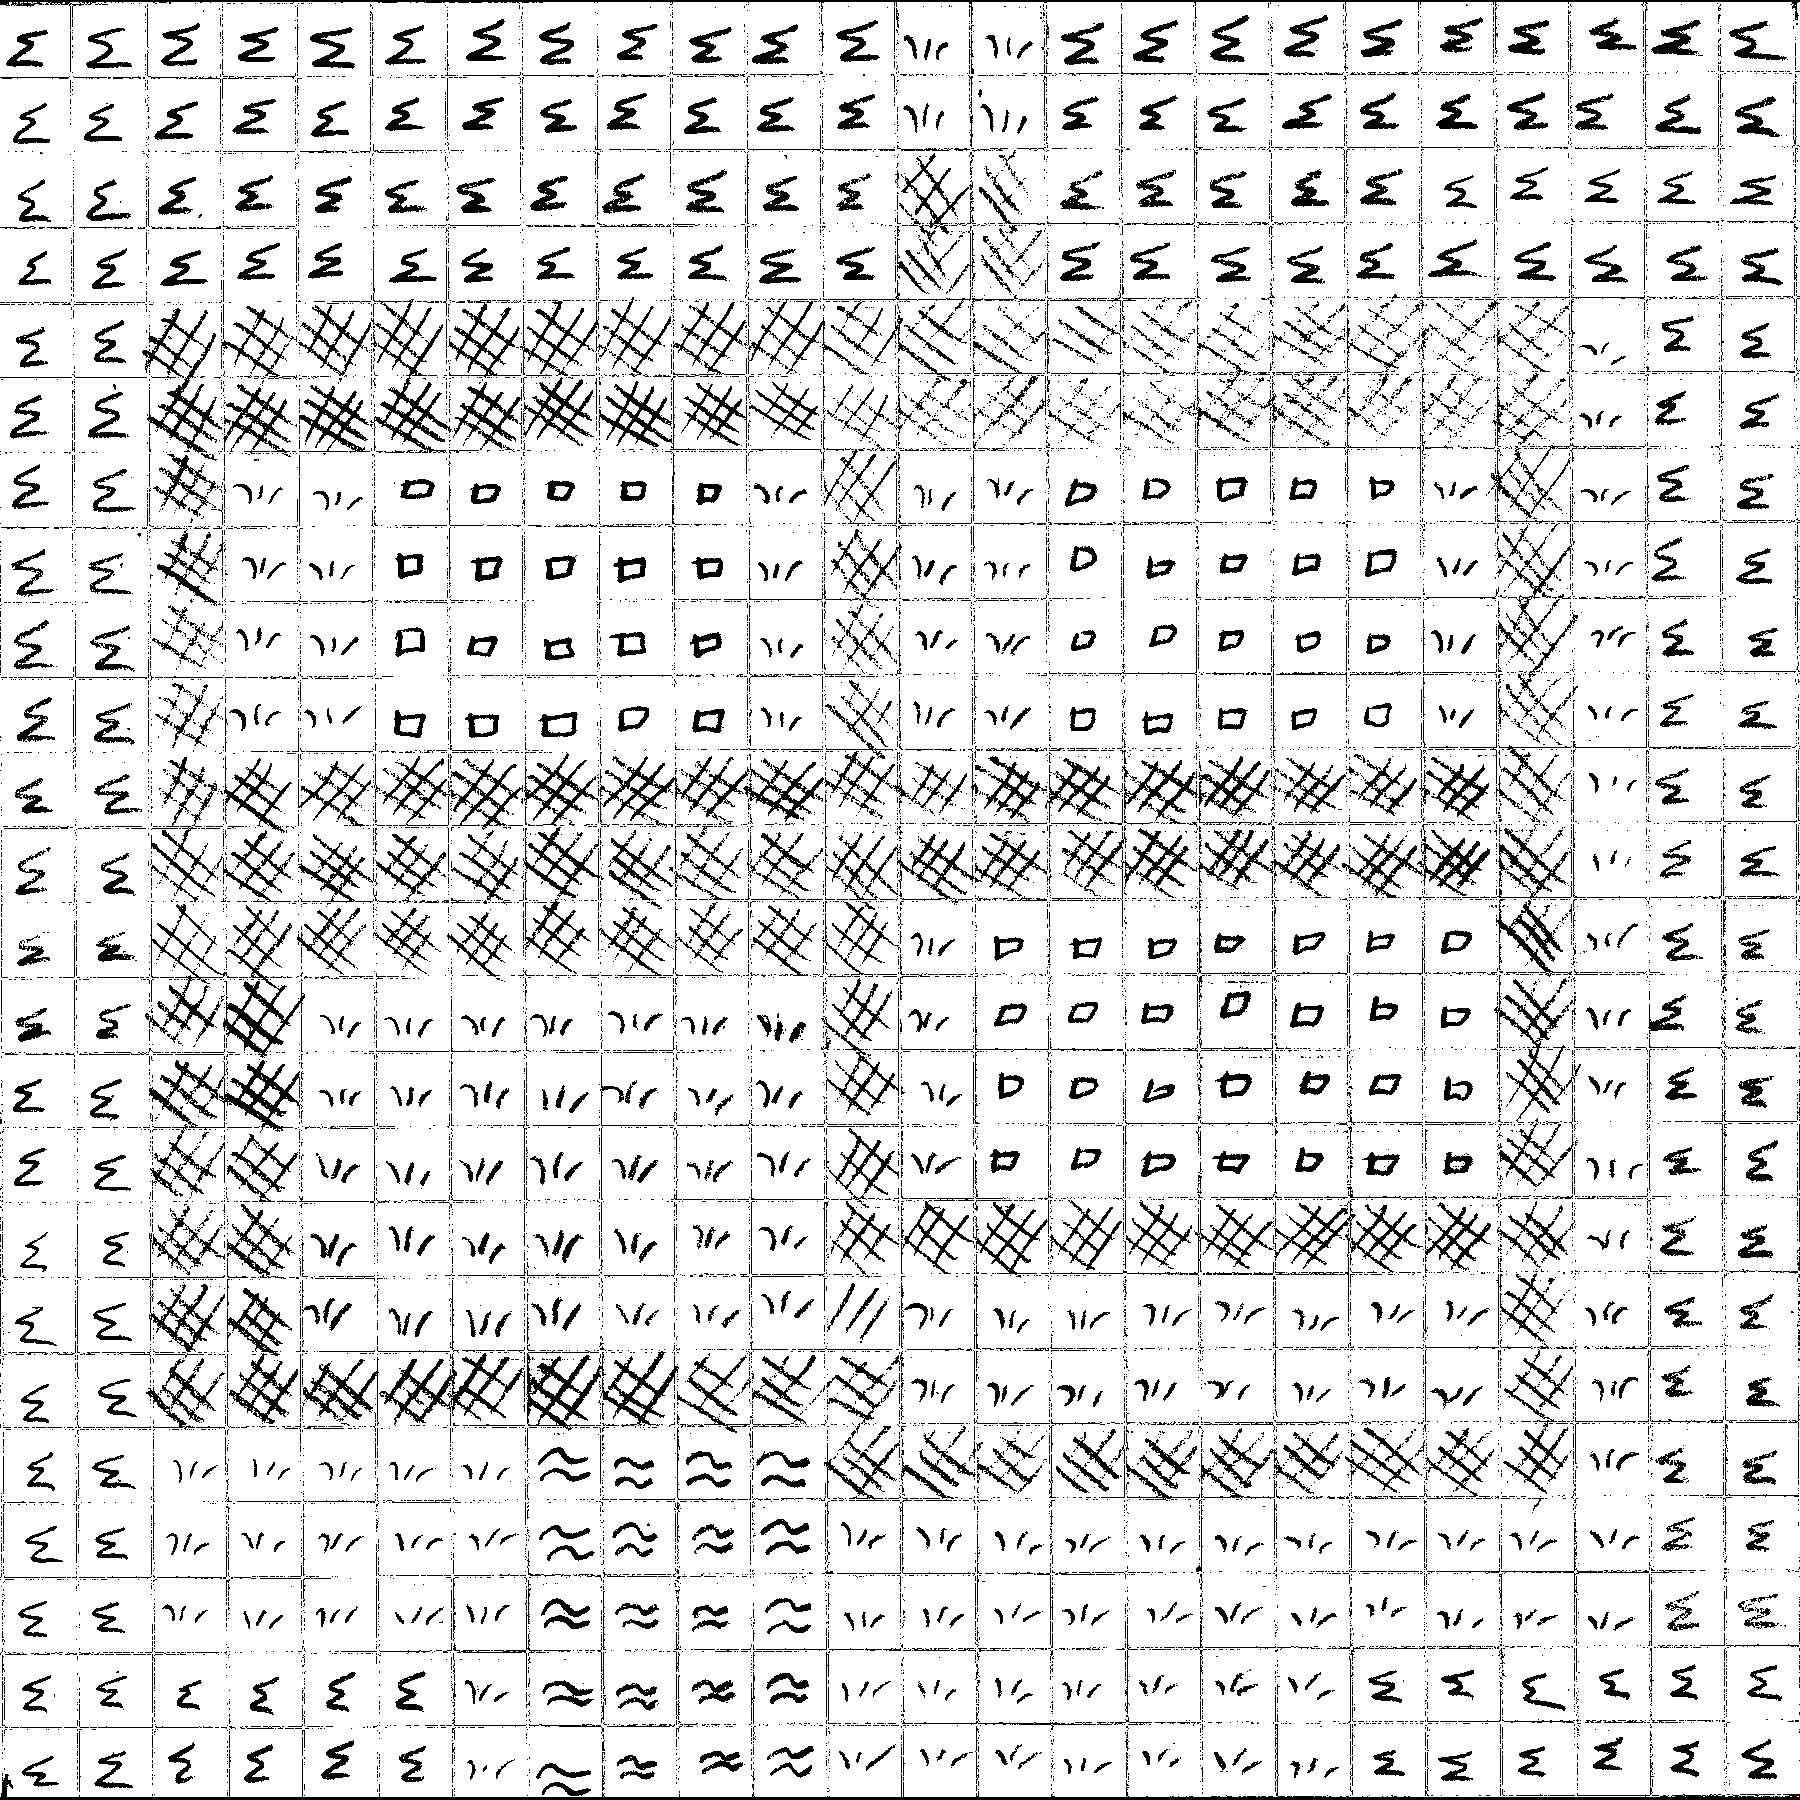
\includegraphics[width=7.5cm, height=7.5cm]{preprocessing-initial}
    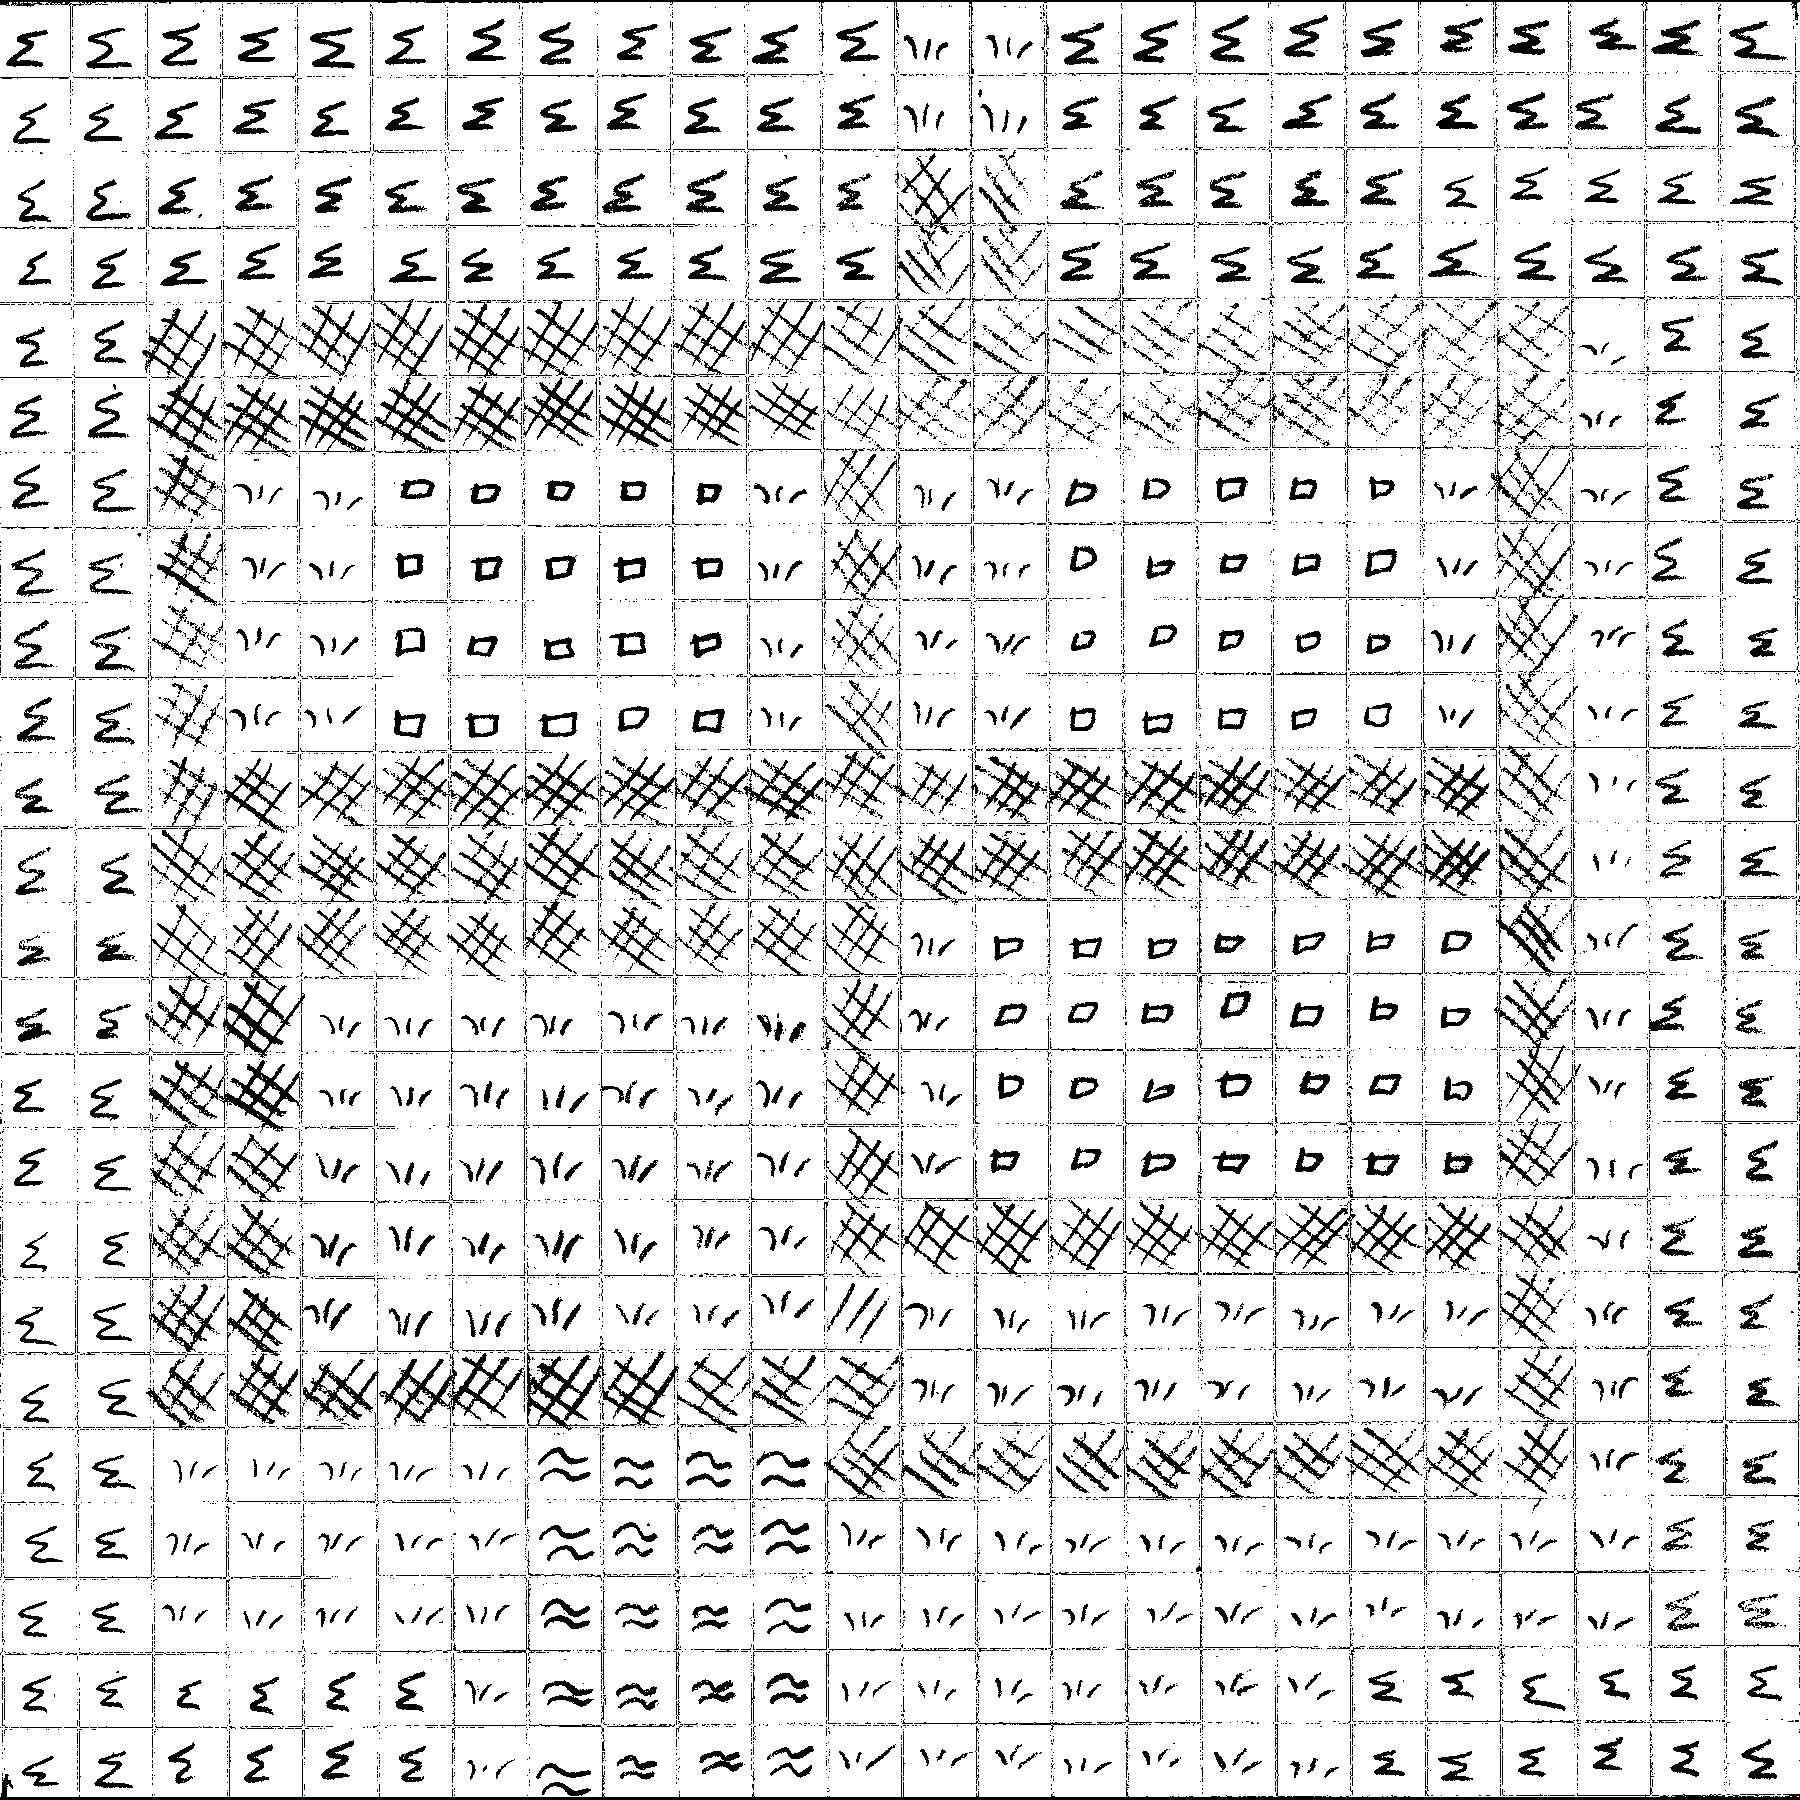
\includegraphics[width=7.5cm, height=7.5cm]{preprocessing-final}
    \label{figure:preprocess}
    \caption{Image before and after preprocessing. Note the increased contrast and faint grid lines}
    \end{center}
\end{figure}

Before analysis, the data must be preprocessed in order to standardize image
properties and reduce the risk of errors in classification. A collection of
scripts are run on each of the maps before classification to rotate, scale, and
remove the blue grid lines using colour filter masks.  Colour information is
removed from the images by converting them to black and white. Contrast is
increased making the symbols appear more pronounced for classification. Each
cell is scaled to a standard 75 by 75 pixels and seperated from the map so that
each cell contains a single symbol.  The results of preprocessing are shown in
Figure \ref{figure:preprocess}

